% !TeX encoding=utf8
% !TeX spellcheck = de_CH_frami

\chapter{BPM in der Domäne "`Internet of Things"'}
Dieses Kapitel beleuchtet \gls{acr:BPM} im Kontext der Domäne \gls{acr:IOT}.

%---------------------------------------------------------------------------------
\section{Die Domäne "`Internet of Things"'}
Das \gls{acr:IOT} hat zum Ziel Dinge aus der realen Welt mit dem Internet und anderen Dingen zu vernetzen. Diese Dinge sollen intelligent und vollständig autonom mit anderen ihnen bekannten und auch unbekannten Geräten und Anwendungen kommunizieren und interagieren können. Durch diese Vernetzung werden die Fähigkeiten der einzelnen Dinge erweitert und im Endeffekt ein Mehrwert für den Anwender geschaffen.

\begin{figure}[H]
 \centering
  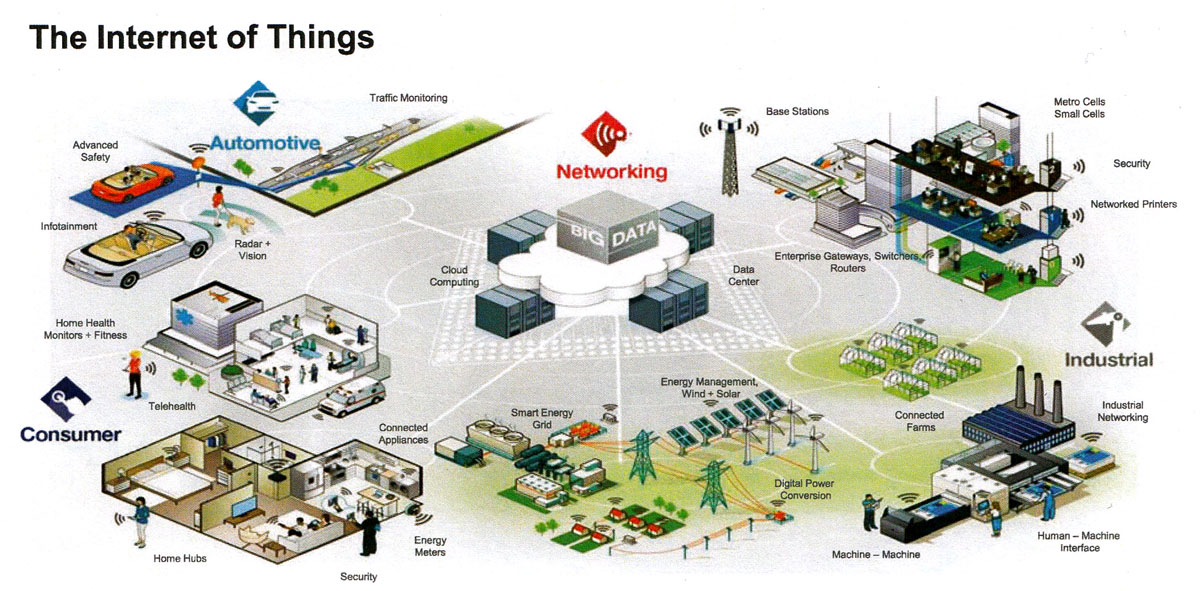
\includegraphics[width=16cm]{./images/freescale_internet_of_things_overview_1}
  \captionsource{Beispielhafte Visualisierung des "`Internet of Things"'}{\url{http://regmedia.co.uk/2014/05/06/freescale_internet_of_things_overview_1.jpg}}
\end{figure}

Bereits früher konnten Dinge und Maschinen selbstständig miteinander kommunizieren. Besonders in den Industriezweigen fand dies Anklang, um die Produktionsanlagen zu überwachen und zu steuern. Das \gls{acr:IOT} stellt nun den nächsten grossen Schritt in dieser Entwicklung dar. Der Hauptaspekt dabei ist die Reduktion der Herstellungskosten und die Miniaturisierung der notwendigen Geräte.

Die Geräte in einem \gls{acr:IOT} können vereinfacht in die Kategorien "`Endgeräte / Things / Dinge"', "`Gateways"' und "`Backend-Systeme"' eingeteilt werden. Die "`Dinge"' stellen die Eckpunkte des \gls{acr:IOT} dar. Gateways stellen typischerweise eine Verbindung zwischen den "`Dingen"' und den Backend-Systemen her. Dabei kann es auch sein, dass ein "`Ding"' gleichzeitig  ein "`Gateway"' darstellt.

An dieser Stelle wird die Domäne \gls{acr:IOT} nicht weiter im Detail beleuchtet. Weitere Hintergrundinformationen und eine Betrachtung im Rahmmen des "`Software Engineering"' sind in der Seminararbeit "`Domain Specific Software Engeineering - Internet of Things"' \cite{E:DBRU:SEM:IOT} zu finden.

\subsection{Herausforderungen \& Problemstellungen}\label{sec:AnalyseIot:ChallangesAndProblems}
Die Domäne \gls{acr:IOT} sieht sich folgenden Herausforderungen und Problemstellungen gegenüber:

\begin{itemize}
\item Verfügbarkeit eines Internet-Zuganges am Einsatz- / Verwendungsort
\item Sicherheit und Datenschutz
\item Tiefe Kosten für Hard- und Software
\item Energieversorgung
\item Energieverbrauch
\item Skalierbarkeit
\item Fehlertoleranz
\item Akzeptanz
\item Robustheit (physisch und logisch)
\item Entdecken von Geräten und Services (Device Discovery)
\item Fernwartung von Geräten und Anwendungen
\item Hersteller Unabhängigkeit / Abhängigkeit (Hardware und Software)
\end{itemize}

Aufgrund der zahlreichen Herausforderungen und Problemstellungen und der daraus resultierenden Komplexität sind grössere Investition in \gls{acr:IOT} nur zu empfehlen, wenn tatsächlich ein Mehrwert geschaffen werden kann.
\newpage
%---------------------------------------------------------------------------------

\section{Prognose für BPM im Kontext von IoT}
Gemäss einem Bericht von Gartner (\cite{E:Gartner:BPM:2015}) sollten die Investitionen in \gls{acr:iBPMS}n im Jahr 2015 um 4.4\% auf 2.7 Milliarden US-Dollar steigen. Im Rahmen der digitalen Transformation überdenken viele Unternehmen ihre Prozesse und Modelle. Einer der 4 genannten Einflussfaktoren ist \gls{acr:IOT}, wobei die "`Dinge"' in die Business Prozesse integriert werden. Dadurch kann sich der Prozess je nach Bedarf den veränderten Bedingungen anpassen. Durch die gemeinsame Orchestrierung mit allen anderen Prozessteilnehmen können Prozessinovationen einfacher umgesetzt werden.

Nach einem anderen Bericht von Gartner aus dem Jahr 2016 (\cite{E:Gartner:BPM:IOT:2020}) werden im Jahr 2020 mehr als die Hälfte aller neuen Business Prozesse und Systeme in irgendeiner Form ein Element von \gls{acr:IOT} beinhalten.


\section{BPM im Kontext von IoT}
Der Einsatzzweck und -nutzen von \gls{acr:IOT} ist stark vom Geschäftsfeld und den Bedürfnissen der Unternehmen abhängig. Daher ist auch eine Kombination / Integration mit \gls{acr:BPM} nicht in jedem Fall sinnvoll, bzw. nutzbringend.

Aktuell werden zwei mögliche Szenarien diskutiert. Eine Partei argumentiert, dass durch die Verbreitung von \gls{acr:IOT} \gls{acr:BPM} nicht mehr adäquat ist und daher mittelfristig verschwinden wird (Siehe \cite{E:LinkedIn:Herring:IOTBPM}). Die andere Partei sieht \gls{acr:BPM} als einen essentiellen und unabdingbaren Baustein für die erfolgreiche Verbreitung von \gls{acr:IOT} (Siehe \cite{E:DataInformed:IOTBPM} oder \cite{E:InformationAge:IOTBPM}). Die Argumente der beiden Parteien werden an dieser Stelle nicht näher beleuchtet, da diese nicht im Kernfokus dieser Arbeit liegen.


Der Einsatz von \gls{acr:BPM} in \gls{acr:IOT} lässt sich in folgende Kategorien unterteilen:
\begin{itemize}
\itemBfText{Privatbereich}
{Beim Einsatz von \gls{acr:IOT} liegt das Hauptaugenmerk auf anderen Punkten, als beim Einsatz in / für ein Unternehmen. Bei einem überwiegenden Teil der Endanwender stehen folgende Faktoren im Vordergrund: Kosten, Funktionsumfang und einfache Bedienung. Es ist in der Regel nicht anzunehmen, dass der Endanwender über technisches Fachwissen verfügt.}

\itemBfText{Kern}
{Diese Kategorie bezeichnet diejenigen Unternehmen für welche \gls{acr:IOT} ein Kerngeschäft darstellt. Diese Unternehmen bieten entweder \gls{acr:IOT}-Lösungen oder Dienstleistungen im selben Bereich an (Hardware und / oder Software).}
 
\itemBfText{Unterstützend}
{Diese Kategorie bezeichnet diejenigen Unternehmen für welche \gls{acr:IOT} als unterstützender Faktor bei essentiellen Geschäftsabläufen / -tätigkeiten eingesetzt wird. Ein Beispiel wäre die Überwachung und Steuerung von Produktionsanlagen in Industriebetrieben.}

\itemBfText{Nice-To-Have}
{Diese Kategorie bezeichnet diejenigen Unternehmen bei welchen \gls{acr:IOT} als "`Nice-to-Have"' im Einsatz ist. Beispiel: Bei einem Finanzdienstleister wurden die Sitzungszimmer so ausgerüstet, dass Online ersichtlich ist, ob es tatsächlich besetzt ist oder nicht.}
\end{itemize} 

Diese Kategorisierung ist nicht abschliessend und lässt sich nicht in jedem Fall anwenden. Beispielsweise ist der Einsatz von \gls{acr:IOT} im Bereich der Gebäudeautomatisierung auch im Unternehmensumfeld sinnvoll. Dies hat jedoch keinen zwingend direkten Einfluss auf das Kerngeschäft. \gls{acr:IOT} bietet jedoch die Möglichkeit viele Effektivitäts- und Effizienzsteigerungen herbeizuführen.



\section{Einfluss und Nutzen}
Wie im Kapitel \ref{sec:Ausg:BPM} \nameref{sec:Ausg:BPM} beschrieben, hat \gls{acr:BPM} das Ziel eine Abstraktion / Vereinfachung der Komplexität herbeizuführen. Da \gls{acr:IOT} einiges an neuer Komplexität mit sich bringt, stellt \gls{acr:BPM} ein geeignetes Mittel dar, um entsprechend einen Teil dieser Komplexität zu reduzieren, beziehungsweise zu abstrahieren. Der Nutzen von \gls{acr:IOT} für eine Branche, beziehungsweise ein Unternehmen, ist sehr unterschiedlich und hängt stark vom angestrebten Ziel ab. Der konkrete Nutzen ist oft auch vom konkreten Kontext abhängig. Zum Beispiel hat eine ans Internet angeschlossene, intelligente Waschmaschine für den Endbenutzer nur einen geringen Zusatznutzen. Für den Hersteller sieht die Situation unter Umständen etwas anders aus. Wenn die Waschmaschine selbstständig feststellen kann, wann bestimmte Teile defekt sind oder in absehbarer Zeit ausgewechselt werden müssen, könnte die entsprechenden Daten direkt an den Hersteller und Wartungstechniker gesendet werden. Dem Hersteller erlaubt dies die Just-In-Time-Produktion der Ersatzteile wodurch entsprechende Kosteneinsparungen möglich sind.



Nachfolgend werden einige Vorteile aufgelistet, welche beim Einsatz von \gls{acr:IOT} in Business Prozessen entstehen:
\begin{itemize}
\item Entstehung neuer Anwendungsmöglichkeiten
\item Erhöhung der Durchgängigkeit von Prozessen
\item Reduktion von Medienbrüchen in Prozessen
\item Konsequente Umsetzung von \gls{acr:BPM}
\item Kosteneinsparungen
\item Effizienz- und Effektivitätssteigerungen
\end{itemize}

Innerhalb von Business Prozessen kann das \gls{acr:IOT} an unterschiedlichsten Stellen eingebunden werden.
\begin{itemize}
\item \gls{acr:IOT}-Endgerät ("`Thing"') liefert Input-Daten für einen Business Prozess.
\item \gls{acr:IOT}-Endgerät ("`Thing"') stellt den Startpunkt / Trigger eines Business-Prozesses dar.
\item \gls{acr:IOT}-Endgerät ("`Thing"') sind Aktoren innerhalb eines Business Prozesses.
\item \gls{acr:IOT}-Endgerät ("`Thing"') sind Endpunkte in einem Business Prozess.
\end{itemize}

Grundsätzlich kann das \gls{acr:IOT} in jedem Teil eines Business Prozesses einen Mehrwert liefern, sofern der entsprechende Bedarf da ist. Es kann gut auch sein, dass der gesamte Business Prozess aus \gls{acr:IOT}-Elementen besteht. Ebenfalls sind Business Prozesse denkbar, welche vollständig auf \gls{acr:IOT} ausgerichtet sind. Dies könnte zum Beispiel bei einem \gls{acr:IOT}-Dienstleister der Fall sein.


\section{Anwendungsmöglichkeiten}
% z.B. SBB: Stellwerkstörung, Spital
\gls{acr:IOT} bietet eine sehr breit gefächerte Palette an Anwendungszwecken und Einsatzzwecken. Diese Palette wird in Zukunft mit der zunehmenden Verbreitung noch grösser werden. Ebenfalls werden sich komplett neue Geschäftsfelder und Möglichkeiten eröffnen.

Nachfolgend werden zwei kurze Beispiel für den Einsatz des \gls{acr:IOT} im Rahmen von (Business) Prozessen aufgezeigt.

\begin{itemize}
\itemBfText{Überwachung der Temperatur in einem Lagerhaus}
{In einem Lagerhaus in welchem die Kühlung, beziehungsweise die Temperatur eine zentrale Rolle spielt könnte mit Hilfe von \gls{acr:IOT} und \gls{acr:BPMN} einiges erleichtert und vereinfacht werden. 

Beispiel: Die einzelnen Produkte sind mit den Informationen ausgestattet, bei welchen Temperaturen diese optimal gelagert werden müssen. Mit Hilfe eines autonomen Fahrzeuges werden die angelieferten Produkte in den entsprechenden Bereich des Lagerhauses verschoben. Gleichzeitig werden die eingelagerten Waren in den entsprechenden Systemen nachgeführt und eine entsprechende Benachrichtigung ausgelöst, dass die Waren eingetroffen sind.

Das Lagerhaus überwacht autonom die Temperatur in den verschiedenen Bereichen des Lagerhauses. Wird eine grössere Abweichung festgestellt oder ein bestimmter Schwellenwert unter- oder überschritten, leitet das System entsprechende Gegenmassnahmen ein. Gleichzeitig wird eine Benachrichtung mit einer entsprechenden Warnung versendet.

Zeigen die eingeleiteten Massnahmen keine Wirkung wird ein weiterer Prozess gestartet. Dieser informiert die zuständige Person über mehrere Kanäle. Die Person kann anschliessend entscheiden, was weiter geschehen soll. Der Prozess bleibt aktiv, bis die Temperatur wieder im korrekten Bereich ist. Im Notfall könnten die Produkte aus dem entsprechenden Bereich automatisch in einen anderen Bereich des Lagerhauses verschoben (zum Beispiel wenn die Kühlung komplett ausfällt). 

Aufgrund der Informationen aus den Prozessen können im Nachgang entsprechende Kennzahlen für weitere Verbesserungen und Optimierungen ermittelt werden.}


\itemBfText{Autonome Produktionsanlage}
{Eine Produktionsanlage könnte durch den Einsatz von \gls{acr:IOT} fast vollständig automatisiert werden.

Beispiel: Durch einen (autonomen) Lieferwagen werden neue Waren angeliefert. Bei der Ankunft meldet sich der Lastwagen selbstständig an. Die Anlage weiss dadurch, was für Waren der Lastwagen anliefert und was mit diesen geschehen soll. 

Das Entladen erfolgt durch einen autonomen Gabelstapler. Dieser kontrolliert den Wareneingang und lagert anschliessend die Waren entsprechend den hinterlegten Informationen im Lagerhaus ein.

Die Produktionsanlage plant die einzelnen Produktionsschritte selbstständig gemäss den zu erreichenden Produktionszielen und Daten ein. Die benötigten Waren werden von der Lage automatisch dem Lager entnommen und entsprechend verbucht. Ist voraussehbar, dass der Warenbestand nicht mehr ausreichen wird um die Produktionsziele zu erreichen, werden automatisch der Nachbestellprozess ausgelöst.

Der aktuelle Fortschritt ist jederzeit ersichtlich und jedes Einzelteil kann im gesamten Produktionsprozess verfolgt werden. Dabei bestimmt das Einzelteil selbst über den nachfolgenden Produktionsschritt. Dazu kennt jedes Einzelteil seine zukünftige Verwendung.

Am Ende des Produktionsprozesses folgen automatische und manuelle Qualitätskontrollen. Wurde diese erfolgreich durchlaufen, werden die fertigen Fabrikate wieder eingelagert und für den Weitertransport vorbereitet. 

Sobald der zuständige Lastwagen für den Transport eintrifft, werden die Waren automatisch verladen und ausgebucht.}

\end{itemize}


\section{Frameworks, Produkte, ...}
Nachfolgend werden einige Frameworks, beziehungsweise Produkte, welche im Bereich \gls{acr:IOT} für die Realisierung und Automatisierung von Business Prozessen verwendet werden können, aufgezeigt und Stichwortartig beschrieben.

\begin{itemize}

\itemBfText{WSO2 IoT Server}{{\small \url{http://wso2.com/products/iot-server/}}\\
WO2 Middleware Plattform, Modular, Erweiterbar, Analytics, BPM-Support, Enterprise Service Bus}

\itemBfText{Pega}{{\small \url{https://www.pega.com/products/pega-7-platform/case-management}}\\
Intelligente Business Process Management Suite}

\itemBfText{Digital Business Platform}{{\small \url{http://www.softwareag.com/corporate/solutions/iot/default.asp}}\\
Analytics, Data-Management, Prozess-Automatisierung, Regeln, Tasks, B2B-Integration}

\itemBfText{OpenIoT}{{\small \url{https://github.com/OpenIotOrg/openiot}}\\
Open Source, Blueprint Middlewar für IoT-Lösungen}

\itemBfText{Internet of Things Cloud Service}{{\small \url{https://www.oracle.com/de/solutions/internet-of-things/index.html}}\\
Analytics, Enterprise Integration, Secure Connectivity, Echtzeitverarbeitung}

\itemBfText{Ritc}{{\small \url{http://www.ritc.io/}}\\
Software as a Service Plattform für IoT, Rule-Engine für Datenverarbeitung}

\itemBfText{Flowthings}{{\small \url{https://flowthings.io/}}\\
Plattform für IoT Lösungen, Cloud basiert, Echtzeit Verarbeitung, Komplexe Eventverarbeitung}

\itemBfText{ubidots}{{\small \url{http://ubidots.com/}}\\
Cloud-Service, Analyse, Aggregierung und Visualisierung von Sensordaten, Definition Regeln und Aktionen}

\itemBfText{zetta}{{\small \url{http://www.zettajs.org/}}\\
API-Frist IoT Plattform, basierend auf Node.js, Open Source}

\itemBfText{Waylay}{{\small \url{http://www.waylay.io/}}\\
Plattform für die Orchestrierung von Enterprise IoT, Analytics, Monitoring, Auslöser und Aktionen}

\itemBfText{Loop (Litmus Automation)}{{\small \url{http://litmusautomation.com/}}\\
IoT Cloud Plattform, High Perfromance und Skalierbarkeit}

\itemBfText{Octoblu}{{\small \url{https://www.octoblu.com/}}\\
Full-STack IoT Plattform, Messaging, Automatisierung, Echtzeitverarbeitung}
\end{itemize}

\newpage
Daneben gibt es auch zahlreiche Produkte, welche spezifisch für die Realisierung von Business Prozessen / Workflows ausgelegt sind. Mit entsprechenden Adaptern oder Erweiterungen können auch diese im Kontext \gls{acr:IOT} verwendet werden.

\begin{itemize}
\itemBfText{Windows Workflow Foundation}{{\small \url{https://msdn.microsoft.com/en-us/library/jj684582.aspx}}\\
.NET Framework von Microsoft, Basis von Sharepoint, Abbildung und Verwaltung von langlebigen Prozessen, Definition in BPMN / XAML }

\itemBfText{nebri}{{\small \url{https://nebrios.com/}}\\
Basiert auf: Python, Docker, Polymer und der Google Cloud Platform, Integration mit anderen Cloud-Diensten, Abbildung von Prozessen und Workflows, Definition in BPMN}

\itemBfText{Decisions}{{\small \url{http://decisions.com/}}\\
Cloud-Lösung oder On-Premise-Lösung, Workflow Engine, Business Rule Engine, Dashboards und Reports, End User Portal, vorgefertigte Integrationsmöglichkeiten in andere Systeme}

\itemBfText{manywho}{{\small \url{https://manywho.com/}}\\
Low Code Development Platform, Workflow, Definition über Designer oder Code, Responsive, Online und Offline, vorgefertigte Integrationsmöglichkeiten}

\end{itemize}


%IBM: http://www.cisco.com/c/en/us/solutions/collateral/enterprise/cisco-on-cisco/t-en-07142014-business-process-ioe.html

% Mögiche Fragestellungen welche in Bezug auf BPMN / IOT zuerst gelöst werden müssen / sollen
%http://enterprise-iot.org/book/enterprise-iot/part-ii-igniteiot-methodology/igniteiot-solution-delivery/building-blocks/iot-technology-profiles/4-middleware/process_efficiency_and_automation/

